\chapter{Auswertung, Fehlerrechnung und Diskussion der Messergebnisse}
\section{Aufgabe 1: Einführung}
Um mit dem Versuchsaufbau vertraut zu werden, wird ein Restgasspektrum Massenbereich \SIrange{1}{51}{amu} unter Standardbedingungen ($E = \SI{65}{eV},I_e =\SI{1}{mA}$) aufgenommen. Ein breiteres Spektrum, wie in der Aufgabe gefordert wird hier nicht betrachtet, da nicht zu erwarten ist das die analysierte Raumluft Moleküle mit $\frac{m}{q} > \SI{51}{\frac{amu}{e}}$ enthält. Das gemessene Spektrum ist  
in Abbildung \ref{fig:MSbreitspektrum} zu sehen, zudem sind die durch einen Savitzky-Golay-Filter geglätteten Daten und die erwarteten Peaks eingetragen. Es ist sichtbar, dass das gemessene Spektrum den Erwartungen entspricht, bis auf den hohen Peak im Bereich von Wasserstoff. Aus Laborerfahrung mit RGAs ist bekannt, das diese im Bereich um \SI{1}{amu} selten sinnvolle Ergebnisse liefern. Desweiteren werden die Peaks der erwarteten Raumluftkomponenten näher betrachtet, diese sind in den Abbildungen \ref{fig:MSWasserPeak}-\ref{fig:MSCO2Peak} im Anhang zu sehen.  

\begin{figure}[H]
    \centering
    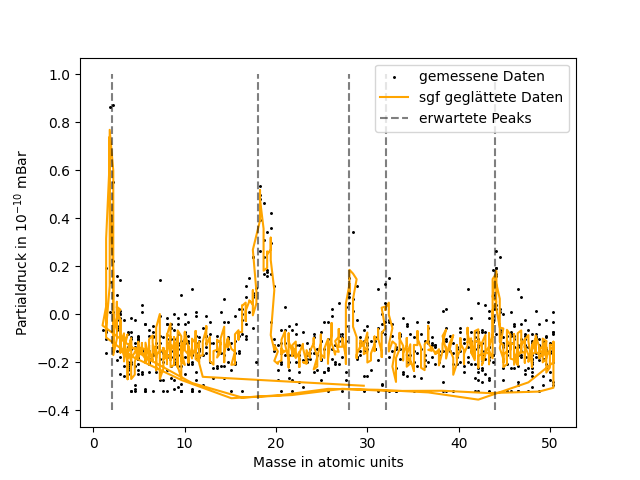
\includegraphics[width=140mm,scale=0.8]{Massenspektrometer/include/MSBreitspektrum.png}
    \caption{Spektrum der Raumluft im Massenbereich \SIrange[]{1}{51}{amu}}
    \label{fig:MSbreitspektrum}
\end{figure}

Der Verlauf des Partialdrucks in Abhängigkeit des Elektronenstroms soll gemessen werden. Dieser ist in Abbildung \ref{fig:MSParDEI} dargestellt. Es ist sichtbar, das der Partialdruck im gemessenen Bereich annähernd linear vom Elektronenstrom abhängt. Die gewählten Standardbedingungen zeigen sich somit als sinnvoll, da sich mit einem maximalem Elektronenstrom von \SI{1}{mA} auch ein maximales Signal bzw. ein maximaler Partialdruck ergibt, was das Signal-Rausch-Verhältnis minimiert. 
\begin{figure}[H]
    \centering
    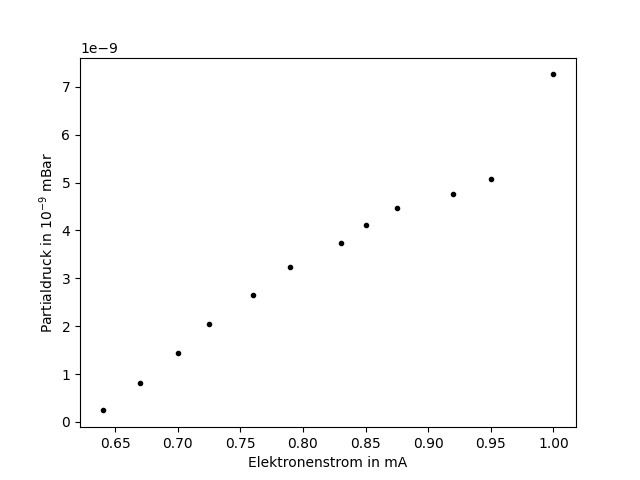
\includegraphics[width=140mm,scale=0.8]{Massenspektrometer/include/MSpardEI.png}
    \caption{Verlauf des Partialdrucks in Abhängigkeit des Elektronenstroms}
    \label{fig:MSParDEI}
\end{figure}

Um das Auflösungsvermögen des Massenspektrometers zu 
berechnen, werden die Peaks aus Abbildungen \ref{fig:MSWasserPeak}-\ref{fig:MSCO2Peak} verwendet. Die Wahl der Definition des Auflösungsvermögen wurde in Kapitel \ref{chapter:MSMassenauflösung} beschrieben. 
Für die gemessenen Peaks ergibt sich somit:

\begin{table}[H]
    \centering
    \caption{Berechnetes Auflösungsvermögen mit $R = \frac{m}{\Delta m}$}
    \begin{tabular}{ccc}
        m in amu & $\Delta$m in amu&  Auflösungsvermögen R\\ \hline
        18.24 & 0.6 &30.4\\
        27.68 & 0.76&36.42\\
        31.36 & 0.76&41.26\\
        43.32 & 1.04&41.65\\\hline
    \end{tabular}
    
    \label{tab:MSAuflösungsvermögen}
\end{table}
In Tabelle \ref{tab:MSAuflösungsvermögen} ist sichtbar, dass das Auflösungsvermögen mit steigender Masse steigt. Dies liegt daran, das die Peakbreite $\Delta m$ unabhängig von der Masse für alle Massen hinreichend konstant ist. 

\section{Aufgabe 2: Austrittsenergie von Argon}

Zur Berechnung der Austrittsenergie von Argon, wird pro Ion von Argon ein Partialdruckspektrum in Abhängigkeit der Beschleunigungsspannung bzw. Elektronenenergie aufgenommen. Dabei ergibt sich ab einer bestimmten Austrittsenergie ein exponetieller Verlauf des Partialdrucks. Um diese Austrittsenergie zu bestimmen, passen wir eine Gerade der Form: $$p(E) = a\cdot E + b$$ an den annäherend linearen Beginn des exponentiellen Graphen an. Mit den angepassten Parametern lässt sich dann der Schnittpunkt mit der x-Achse bilden: $$E(p=0) = -\frac{b}{a}$$ was der Austrittsenergie entspricht. Leider ist ein Datensatz dieser Aufgabe verloren worden, sodass nur die Austrittsenergie des einfach ionisierten Argons bei \SI{40}{amu} bestimmt werden kann. Für zweifach ionisiertes Argon bei \SI{20}{amu} würde die Analyse analog erfolgen. 

In das gemessene Spektrum des einfach ionisierten Argons wird eine Gerade angepasst: 
\begin{figure}[H]
    \centering
    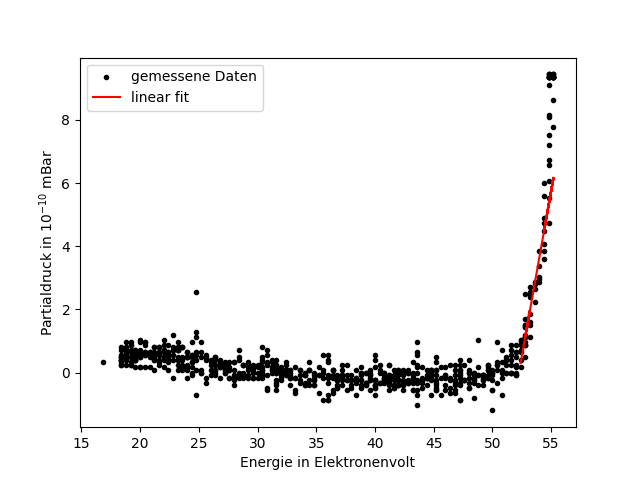
\includegraphics[width=140mm,scale=0.8]{Massenspektrometer/include/MSArgon1Ion.png}
    \caption{Spektrum des Partialdrucks von einfach ionisiertem Argon in Abhängigkeit der Elektronenergie}
    \label{fig:MSParDEI}
\end{figure}
Unter der Annahme von einer Unsicherheit von \SI{5}{\%} auf den Partialdruck ergibt die Anpassung:
$$a = \SI{2.09(2)e-10}{\frac{mbar}{eV}}, b= \SI{-1.09(1)e-8}{mbar}$$
Die Austrittsenergie ergibt sich somit unter Verwendung von gaußscher Fehlerfortpflanzung zu:
$$E_{aus} = \SI{53.25(0.76)}{eV}$$
Zum Literaturwert, $E_{lit(Ar^+)}= \SI{15.76}{eV}$\cite{VorbereitungsMappe} besteht eine erheblicher Differenz, welche nicht im Fehlerbereich enthalten ist. Vermutlich wurde der falsche Teil des Spektrums an eine Gerade angepasst.   

\section{Aufgabe 3: Dissoziationsenergien von Stickstoff}

Die Dissoziationsenergien von Stickstoff lassen sich unter Kentnis der Ionisationsenergie von atomarem Stickstoff aus den Austrittsenergien berechnen. Zur Berechnung dieser, wird analog zu Aufgabe 2 vorgegangen. 
